\chapter{Background}

In this chapter, we introduce some of the techniques we use in the following
chapters. 
%
In particular, we describe a form of supervised learning, classification, and of
unsupervised learning, clustering.
%
We also describe the use of {\em word embeddings}, in particular, the modern use
of neural network-based word embeddings, such as {\em word2vec} and {\em
fastText}.


\section{Supervised learning: Classification}

The basic premise of learning from data is the use of a set of observations to
uncover an underlying process~\cite{Abu-Mostafa:2012:LD:2207825}. 
%
More formally, a way to see this is finding a function that optimizes certain
score, based on the available data. 
%
This function can be seen as an approximation of the real, unknown function
that describes the process that generates the data.

%%

When the {\em training data} (the available data) contains explicit examples of
what the correct output should be, then we are within the supervised learning
setting.
%
In this setting, classification is the process to assign a certain {\em label}
to an observation, or data point, in order to categorize it into a certain class
or category.
%
A {\em classifier} is a particular instance of the process, which can be {\em
trained} from a set of previously labeled observations in order to set its
appropiate parameters.
%
The output of a classifier applied to an observation is the label corresponding
to that observation (Figure~\ref{background:fig:clf-ex}).
%
Formally, a classifier is a function $h: \mathcal{D} \rightarrow \{0, 1, \ldots,
n\}$ from a domain $\mathcal{D}$ to a set of classes, or class labels, which
tries to approximate to the {\em real} function $f$.
%
A {\em binary classifier} is a function restricted to only two labels, $h:
\mathcal{D} \rightarrow \{0, 1\}$.
%
The training process of a classifier corresponds to find a function $h$ from a
{\em hypothesis set} $\mathcal{H}$ which contains all possible functions based
on the selected {\em model}.
%
For example, $\mathcal{H}$ would be all quadratic functions $h(x) = ax^2 + bx +
c$, and the goal is to find the correct set of parameters $(a, b, c)$ that make
$h$ fit the training data.
%
An error measure that is commonly used is the squared error: $e(h) =
(h(\vect{x}) - f(\vect{x}))^2$.
%
As we do not know $f$, the error measure is only an approximation of the real
error, which is called {\em in-sample error}, while the real error is called
{\em out-of-sample error}.
% 
There are models that estimate bounds for which the in-sample error can
approximate the out-of-sample error.
%
In the binary setting, the Vapnik–Chervonenkis (VC) dimension~\cite{Vapnik2015}
is an estimation on how well a function $h$ from a hypothesis set can fit a set
of data points, based on the characteristics of $\mathcal{H}$ and the number of
data points.

%
\begin{figure}
    \centering
    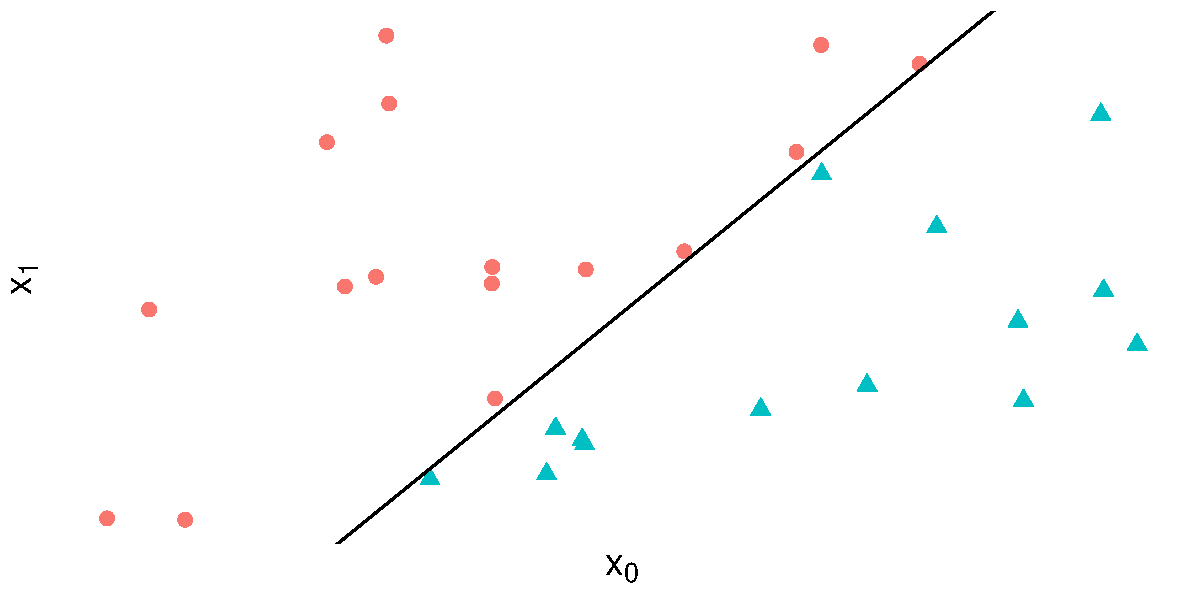
\includegraphics[width=.8\textwidth]{figures/background/classification-example}
    \caption{Example of classification as a decision boundary.}
    \label{background:fig:clf-ex}
\end{figure}%


\paragraph{Linear models.} The linear model is the family of functions (or
hypothesis set) defined as $h(\vect{x}) = \vect{w}^\customT\vect{x}$, where
$\vect{w} \in \mathbb{R}^\textit{d}, \textit{d} > 0$ is a vector of weights, and
$\vect{x}\in \mathbb{R}^\textit{d}$ is an observation. 
%
The {\em perceptron} is defined as $h(\vect{x}) =
\text{sign}(\vect{w}^\customT\vect{x})$, which is the foundation of several
linear models and neural network models.

%%

The perceptron uses a hard threshold on the signal $s =
\vect{w}^\customT\vect{x}$ by taking the sign of $s$ in order to perform linear
classification.
%
{\em Linear regression} outputs a real value by using the signal $s$ as the
output, $h(\vect{x}) = \vect{w}^\customT\vect{x}$.
%
{\em Logistic regression} restricts the output to the range $[0, 1]$, making
it interpretable as a probability: $h(\vect{x}) =
\theta(\vect{w}^\customT\vect{x})$, where $\theta$ is the so-called logistic
function, $\theta(s) = \frac{e^s}{1 + e^s}$.
%
There are several other linear models, which we will not mention in this brief
summary, but some of them can be studied
online\footnote{\url{https://scikit-learn.org/stable/modules/linear_model.html}
(Accessed: April 8, 2019)}.

%%

There are different learning algorithms in each case. 
%
For the perceptron, there is the {\em Perceptron Learning Algorithm} and the
{\em Pocket Algorithm}~\cite{Abu-Mostafa:2012:LD:2207825}. 
%
For the linear regression, a exact analytic expression can be derived by
minimizing the in-sample error, $E_{\text{in}}(h) = \frac{1}{N} \sum_{n=1}^{N}
(h(\vect{x}_n) - y_n)^2$, where $y_n = f(\vect{x}_n)$ is the label of the $n$-th
observation.
%
For logistic regression, the {\em gradient descent algorithm} provides a way to
find a local optimum for the in-sample error $E_{\text{in}}(h)$, which is
defined as the cross-entropy measure between $h(\vect{x})$ and $y$. 

%%

Gradient descent is a general technique for minimizing a twice-differentiable
function. 
%
It is performed by computing the gradient of the in-sample error $\nabla
E_{\text{in}}(h)$, and ``moving'' the weight vector according to the direction
of the gradient, $\vect{w}_{t+1} = \vect{w}_t - \eta\nabla E_{\text{in}}(h)$.
%
There are several strategies to stop the iteration $t$, such as doing it until
the change is small, a fixed number of times, when the error is small enough, or
a combination of the above.
%
The magnitude of the movement is given by the parameter $\eta$, or {\em learning
rate} which is usually a fixed value.

\paragraph{Neural network models.} 


\paragraph{Evaluation.}

The standard workflow of training a classifier involves splitting the available
data into a {\em training set} and a {\em test set}. 
%
\todo[inline]{escribir sobre holdout y CV} 

The most common metric to evaluate the effectiveness of a classifier is the {\em
accuracy}, the amount of correctly classified observations over the total amount of
observations.

\begin{equation}
    \text{Accuracy} = \frac{\text{\#(correctly\ classified\ observations)}}{N}
\end{equation}

Where $N$ is the total amoun of observations being classified.

Accuracy does not account for an imbalance in the class distribution.
%
For example, when there are two classes, and they are split into 99\% class $0$
and 1\% class $1$, then it is easy to obtain an accuracy of $0.99$ by
classifying everything as class $0$.
%
The notion of {\em Precision} and {\em Recall} take into account two types of
error of a classifier.

\begin{equation}
    \text{Precision}_c = \frac{\text{\#(observations\ correctly\ classified\ as\ } c \text{)}}{ \text{\#(observations\ classified\ as\ } c \text{)} }
\end{equation}

\begin{equation}
    \text{Recall}_c = \frac{\text{\#(observations\ correctly\ classified\ as\ } c \text{)}}{ \text{\#(observations\ of\ class\ } c\text{)} } 
\end{equation}

The related errors are the {\em false positives} (when an observation is
incorrectly classified as the target class) or FP, the {\em false negatives}
(when an observation is incorrectly classified as something that is not the
target class), or FN. 
%
When an observation is correctly classified as the target class, we say it is a
{\em True Positive}, TP, and when it is correctly classified not as the target
class, a {\em True Negative}, or TN.
%
Now we can re-write the definitions of accuracy Accuracy, precision $P$, and recall
$R$:

\begin{align}
    \text{Accuracy} &= \frac{\cTP + \cTN}{\cTP + \cFP + \cFN + \cTN} \\
    P &= \frac{\cTP}{\cTP + \cFP} \\
    R &= \frac{\cTP}{\cTP + \cFN} 
\end{align}

A single measure that trades off precision versus recall is the {\em F-score} or
{\em F measure}, which is the weighted harmonic mean of precision and recall:

\begin{equation}
    F = \frac{1}{\alpha\frac{1}{P} + (1-\alpha)\frac{1}{R}} = \frac{(\beta^2+1)PR}{\beta^2P+R} \text{\ \ where\ \ } \beta^2 = \frac{1-\alpha}{\alpha}
\end{equation}

where $\alpha \in [0, 1]$ and thus $\beta^2 \in [0, \infty]$. 
%
The default {\em balanced F measure} equally weights precision and recall, which
means $\alpha=1/2$ or $\beta=1$.
%
It is commonly written as $F_1$.
%
In this case, the formula translates to:

\begin{equation}
    F_1 = \frac{2PR}{P+R}
\end{equation}

%%

The {\em confusion matrix} is a specific table layout that shows the performance
of a classifier.
%
Each row of the matrix represents the instances of the actual class, while each
column represents the instances in the predicted classes.
%
When there are two classes, the cells of the matrix represent the TP, FP, FN,
and TN of the classifier results.
%
Table~\ref{tab:background:example-conf-matrix} shows an example of a confusion
matrix with three classes.

%%

Another concept sometimes used in the evaluation is the {\em ROC
curve}\footnote{Or Receiver Operating Characteristics curve.}. 
%
The ROC curve plots the {\em true positive rate}, {\em sensitivity} or simply
recall, against the {\em false positive rate} or $(1 - \mathit{specificity})$.
%
The false positive rate is given by $\cFP/(\cFP + \cTN)$.
%
The true positive and false positive rates are computed based on different
threholds imposed to the decision boundary of a classifier, for example, at the
threshold of a logistic regression classifier when deciding if an observations
belongs to one or the other class.


\begin{table}[]
    \centering
    \begin{tabular}{@{}llll@{}}
    \toprule
    Actual / Predicted & \textit{Class 0} & \textit{Class 1} & \textit{Class 2} \\ \midrule
    \textit{Class 0}   & \textbf{10}      & 4                & 6                \\
    \textit{Class 1}   & 2                & \textbf{14}      & 0                \\
    \textit{Class 2}   & 4                & 23               & \textbf{9}       \\ \bottomrule
    \end{tabular}
    \caption{Example of confusion matrix for a classifier with three classes.}
    \label{tab:background:example-conf-matrix}
    \end{table}

\section{Unsupervised learning: Clustering}

Clustering algorithms group a set of documents into subsets or {\em
clusters}~\cite{manning2010introduction}.
%
The goal of the algorithms is to produce clusters that are internally coherent,
while very different from each other.
%
Clustering is the most common form of unsupervised learning, when we do not have
the exact labels corresponding to each observation. 
%
In this case, it is the features in the data which will correlate to the labels.
%
Our goal is to replicate the distinction that a human observer would impose on
the data.


\paragraph{K-Means.} 
%
K-Means is a partitional clustering algorithm which assigns each observation to
exactly one cluster.
%
The objective of K-Means~\cite{lloyd1982least} is to minimize the average
squared Euclidean distance of documents from their cluster
centers~\cite{manning2010introduction}.
%
A cluster center is defined as the mean, or {\em centroid} $\vect{\mu}$ of the
observations in a cluster $\omega$:

$$\vect{\mu}(\omega) = \frac{1}{|\omega|} \sum_{\vect{x} \in \omega} \vect{x}$$

K-Means aims to minimize the {\em sum of the squared error}, or
SSE\footnote{Also called {\em Residual Sum of Squares}, or RSS.}, the squared
distance of each vector from its centroid summed over all vectors:

$$ \text{SSE}_k = \sum_{\vect{x} \in \omega_k} |\vect{x} - \vect{\mu}(\omega_k)|^2 $$

$$ \text{SSE} = \sum_{k = 1}^K \text{SSE}_k, $$

where $K$ is the total amount of clusters, and $\omega_k$ is the $k$-th cluster.

Initially, the algorithm selects the initial $K$ centroids randomly.
%
Then it moves the centers around in space in order to minimize SSE.
%
Iteratively it reassigns the observations to the cluster with the closest
centroid, and recomputes each centroid based on the current members of its
cluster. 

The algorithm is as follows: \vspace{.3cm}

\begin{algorithmic}
\STATE {\scshape K-Means}$(\{\vect{x}_1, \ldots, \vect{x}_N\}, K)$
    \STATE $(\vect{s}_1, \vect{s}_2, \ldots, \vect{s}_K) \gets$ {\scshape SelectRandomSeeds}$(\{\vect{x}_1, \ldots, \vect{x}_N\}, K)$
    \FOR{$k \gets 1\ \TO\ K$} \STATE $\vect{\mu}_k \gets \vect{s}_k$ \ENDFOR
    \WHILE{stopping\ criterion\ has\ not\ been\ met}
        \FOR{$k \gets 1\ \TO\ K$}
            \STATE $\omega_k \gets \{\}$
        \ENDFOR
        \FOR{$n \gets 1\ \TO\ N$}
            \STATE $j \gets \text{arg} \min_{j'} |\vect{\mu}_{j'} - \vect{x}_n|$
            \STATE $\omega_j \gets \omega_j \cup \{\vect{x}_n\}$
        \ENDFOR
        \FOR{$k \gets 1\ \TO\ K$}
            \STATE $\vect{\mu}_k \gets \frac{1}{\omega_k}\sum_{\vect{x}\in\omega_k}\vect{x}$
        \ENDFOR
    \ENDWHILE
    \RETURN $\{\vect{\mu}_1, \ldots, \vect{\mu}_K\}$
\end{algorithmic}

K-Means has some considerations to be taken into account:

\begin{itemize}
\item {\bf Termination condition.} 
%
We can apply one of the following termination conditions.
%
(i) a fixed number of iterations $I$ has been completed; 
%
in this case, the quality of the clusters can be compromised because an
insufficient number of iterations.
%
(ii) the assignment of data points to clusters does not change between
iterations; 
%
this can yield a good clustering solution, except for a bad local minimum.
%
(iii) the centroids $\vect{\mu}_k$ does not change between iterations;
%
this is equivalent to the assignment not changing.
%
(iv) terminate when SSE falls below a certain threshold.
%
(v) terminate when the decrease of SSE falls below a certain threshold, meaning
that we are close to convergence.
%
A common strategy is to combine criterions, such as a maximum number of
iterations, a threhold on the value or decreasing rate of SSE, etc.

\item {\bf How to choose the initial seeds.} 
%
Effective heuristics for chosing the initial seeds include:
%
(i) excluding outliers from the seed set;
%
(ii) trying multiple starting points and choosing the best clustering (in terms
of SSE);
%
(iii) obtain the seeds from another methods, such as hierarchical clustering.

\item {\bf Selecting the number of clusters $K$.}
%
One of the most popular heuristics to choose the number of clusters $K$ on
K-Means, when there is no previously conception of what the number should be, is
as follows.
%
For every value of $K$ in a chosen range, compute K-Means $t$ times (e.g. $t =
10$), each with a different initialization of seeds, and take the minimum value
of SSE of the $t$ runs.
%
Then, we can inspect the values of SSE for every $K$ and find the ``knee'' or
``elbow'' in the curve: the point where successive decreases in SSE become
noticeable smaller.
%
This is known as the {\em elbow method} for selecting the number of clusters.
%
Another criterion imposes a penalty on the number of clusters.
%
For example, the elbow method could suggest different values of $K$, and we
would prefer a smaller value.
%
The criterion uses a weighting factor $\lambda$ on the number of clusters: $K =
\text{arg min}_K [\text{SSE}_{\text{min}}(K) + \lambda K]$.
%
This is similar to the regularization factor in classification.
%
The value of $\lambda$ can be derived empirically or use a value that was being
shown to be effective in the domain of study.
\end{itemize}

\paragraph{Evaluation of clustering.} 
%
Criterions on clustering quality involve two perspectives: internal and external
evaluation.
%
Internal evaluation assesses the characteristics that objective functions in
clustering try to attain, such as having high intra-cluster similarity (elements
within a cluster are similar), and low inter-clustering similarity (elements
from different clusters are dissimilar).
%
On the other hand, when we have a {\em gold standard}, or a set of classes
corresponding to the ``real'' clusters, we can perform external evaluation, by
comparing our clustering solution to the gold standard.

%%

In the case of K-Means, the value of the SSE is itself an internal criterion,
because we are validating our solution in terms of the intra-cluster similarity.
%
One can use both intra and inter-cluster similarity to judge the quality of the
clustering. There are other measures, such as the Silhouette
value~\cite{rousseeuw1987silhouettes}, and the Davies-Bouldin
index~\cite{davies1979cluster}.

%%

In this section we will describe the following external evaluation measures for
clustering: {\em purity}, {\em normalized mutual information}, and the {\em rand
index}.

%%

To compute purity, each cluster is assigned to the class which is most frequent
in the cluster, and then the accuracy of this assignment is measured by counting
the number of correctly assigned observations.
%
Formally:

$$ \text{purity}(\Omega, \mathbb{C}) = \frac{1}{N} \sum_{k}^K \max_j |\omega_k \cap c_j|$$

where $\Omega = \{\omega_1, \omega_2, \ldots, \omega_K\}$ is the set of clusters
and $\mathbb{C} = \{c_1, c_2, \ldots, c_J\}$ is the set of classes (the gold
standard).

%%

Bad clustering solutions have values of purity close to 0, and perfect
clustering has a value of 1. 
%
However, as $K$ increases, the value of purity tends to increase as well. 
%
For example, a purity of 1 is achieved when every cluster has only one
observation.

%%

To make a tradeoff between the number of clusters and the quality of the
clustering solution, we can use normalized mutual information, or NMI.
%
NMI is defined as follow:

$$ \text{NMI}(\Omega, \mathbb{C}) = \frac{I(\Omega; \mathbb{C})}{[H(\Omega) + H(\mathbb{C})]/2} $$

$I$ is mutual information, defined as 


\begin{align}
    I(\Omega; \mathbb{C}) &= \sum_k \sum_j P(\omega_k \cap c_j) \log \frac{P(\omega_k \cap c_j)}{P(\omega_k) P(\cap c_j)} \label{eq:mutual-info} \\ 
    & = \sum_k \sum_j \frac{|\omega_k \cap c_j|}{N} \log \frac{N|\omega_k \cap c_j|}{|\omega_k| |c_j|} \label{eq:mutual-info2}
\end{align}



where $P(\omega_k)$, $P(c_j)$, and $P(\omega_k \cap c_j)$ are the probabilities
of the observations being in cluster $\omega_k$, class $c_j$, and in the
intersection of $\omega_k$ and $c_j$, respectively. 
%
Equation~\ref{eq:mutual-info2} is equivalent to \ref{eq:mutual-info} for maximum
likelihood estimates of the probabilities, that is, the relative frequency.
%
$H$ is entropy, defined as 

\begin{align}
H(\Omega) &= - \sum_k P(\omega_k) \log P(\omega_k) \label{eq:entropy} \\
&= - \sum_k \frac{|\omega_k|}{N} \log \frac{|\omega_k|}{N} \label{eq:entropy2}
\end{align}
    
The intuition behind mutual information (MI) is that it measures the amount of
knowledge we gain about the classes when we know what the clusters are. 
%
When the clustering assignment is random, we gain no new knowledge, and MI is 0.
%
It suffers the same problem as purity, so MI is maximum when the perfect
clustering is also one cluster per observation.
%
For that, NMI normalizes MI using entropy.

%%

Entropy tends to increase with the number of clusters. 
%
In this case, NMI is low when $K = N$, because $H(\Omega)$ is maximum when $K =
N$. 
%
The denominator $[H(\Omega) + H(\mathbb{C})]/2$ is a tight upper bound on MI, so
NMI ranges between 0 and 1.

%%

Another view on clustering is to consider the process as a series of decisions,
where we decide for each pair of observations, if they belong to the same
cluster or not.
%
We want to assign observations to the same cluster if they are similar (or if
they both belong to the same class).
%
So, if we assign a pair of similar observations to the same cluster, it is
considered a True Positive (TP). 
%
A pair of dissimilar observations assigned to different clusters is a True
Negative (TN).
%
Likewise, two similar observations in different clusters correspons to a False
Negative (FN), and two dissimilar observations in the same cluster a False
Positive (FP).
%
The Rand Index (RI) measures the percentage of correct decisions, or just the
accuracy.

\begin{equation}
    \text{RI} = \frac{ \text{TP} + \text{TN} }{ \text{TP} + \text{FP} + \text{FN} + \text{TN}}
\end{equation}

From this representation we can define the equivalent to precision, recall, and
F-score.

\section{Neural Network-based Word Embeddings}